\section{Interviews: Expert \& Novice Differences in Comic Drawing Process}
\label{sec:shown_ints} 

\subsection{Method: Interviewing Expert Artists \& Novices}
Differences in experts and novices have been well-studied in various domains from chess \cite{Chase1973} to physics \cite{chi1981categorization}; experts are able to contextually apply different high-level strategies to their work while novices often focus on details. We wanted to understand where novices struggle most in the domain of drawing comics to learn about the types of examples that would be most beneficial to support in an adaptive creativity support tool. 
We interviewed and observed nine expert artists and nine novices as they performed a comic-drawing task. We chose comics as a domain because most people would likely benefit from examples when engaging in the intersection of verbal and visual storytelling \cite{abel2008drawing,eisner2008comics, mccloud2006making} and because drawing comics requires only pen and paper at a minimum. 

We recruited experts from the freelance site Upwork, and novices through social media posts. Experts had formal art training and professional experience in making comic strips. We recruited novices who had a familiarity with comics, but no experience making comics and no formal education or professional experience in art. Over the course of an hour, participants drew a four-panel comic for one of three randomly given prompts: 

\begin{itemize}
\item{\textsc{Penguin}: a man befriends a penguin because of shared interests,}
\item{\textsc{Aliens}: aliens invade Earth during the 2020 global pandemic quarantine, and} \item{\textsc{Character}: a woman is upset at her date because he doesn't know who her favorite television or movie character is.} 

\end{itemize}
We asked participants to think aloud as they drew and asked questions about their process. After participants finished drawing, we asked them what they found easiest and hardest about making their comics, what the feel is the most important part of comics, and what type of help they feel would be most useful. All interviews took place on the Zoom video conferencing platform, and participants were allowed to draw digitally or use pen and paper. Experts received USD \$60 payment for their participation; novices received a \$25 gift card.

\begin{figure*}
  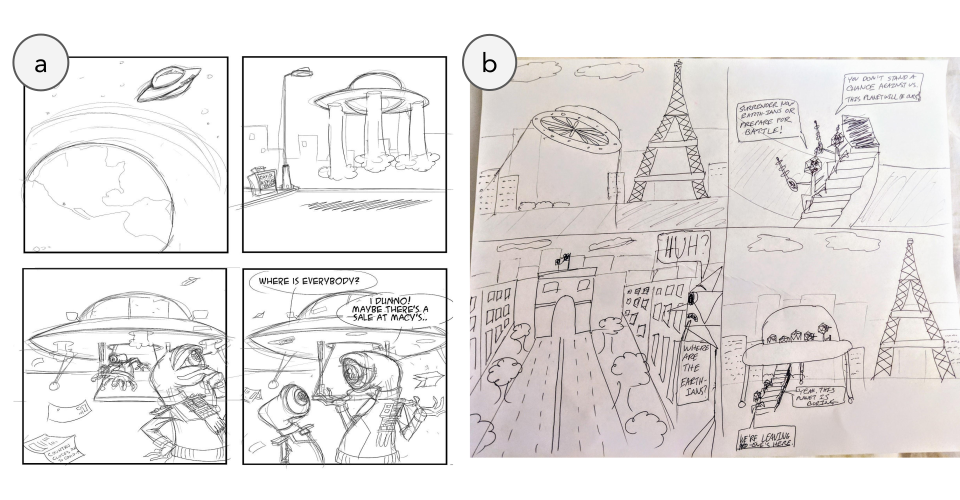
\includegraphics[width=\textwidth]{shown/figures/study1.png}
  \caption{Examples of an a) expert and b) novice comic for the \textsc{Aliens} prompt: aliens invade Earth during the 2020 global pandemic quarantine.}
  \label{fig:study1}
\end{figure*}

\subsection{Results}

\subsubsection{Experts Focus on Story \& Composition}
All nine expert artists expressed that story and composition are the most important parts of a comic: ``\textit{It’s all about composition because if you can’t understand how a comic moves, the narrative kind of decomposes}'' (Expert 4). Experts stressed that good drawing skills alone do not make a comic interesting, explaining that writing is more critical to a good comic than the fidelity of its drawings: ``\textit{I feel like the most important part is the composition of each panel because you can have great illustration..., but if the composition leads to just a random object in the background that isn’t important to the story..., the audience is going to miss something}'' (Expert 2).
Expert 8 similarly said, ``\textit{The most important thing is the writing because if you’re a good artist, but your writing stinks, you’re not going to make it. But you can have awesome writing and stick figures and make a million bucks, so to speak}.'' 

To achieve their narrative goals, experts mentioned using composition concepts and rules to help establish the flow and message of the comic. Expert 5 stated, ``\textit{There’s pretty simple rules of composition, you know, thirds, rhythm, all that stuff. They kind of help lead you to the subject’s eyelines.}'' As in prior work on expert drawing strategies \cite{Edwards1979,Poore1967}, experts drew rough sketches to rapidly outline their ideas. These quick sketches helped them evaluate their work in terms of visual concepts like composition, as well as narrative concepts like flow and pacing. For example, Expert 6 said, ``\textit{So I just plan out how I want it to look. And, you know, once you're done with something you're always like, ‘Oh, I can make that better. I can make it nicer.’ To get the general gist, we're going to see what they're doing, and etcetera.}'' Expert 1 similarly explained, ``\textit{And at this point, I'm still kind of planning stuff out. So I'm not really drawing what might be there, just kind of a reference. So I guess laying it out.}'' Three experts talked about typically creating thumbnail sketches to ideate panel compositions: ``\textit{I'll do like four or five different little sketches or thumbnails of what I think are good for the theme that I chose in my brainstorming session}'' (Expert 7). After a rough sketch, experts refine their sketch by adding in details, then move into a final inking stage to finish drawing their comic. Expert 5 said that doing a final drawing was the quickest part of the process because the idea in mind was already on paper. In general, experts spent most of their time on exploration and iteration while focusing on high-level elements like composition and flow, enabling them to finish drawing their comics quickly and simply. 

\subsubsection{Novices Focus on Details}
Verbally, novices also expressed the view that narrative arc is paramount: \textit{e.g.}, ``\textit{[The most important thing is] conveying the story I want to tell in as clear a way as possible}'' (Novice 8). Despite this, novices time allocation favored detailed drawings over composition and flow. For example, one novice drew the details of a character before deciding on story plot or composition. Another spent nearly 10 minutes drawing a person starting from the feet up in one panel, leading them to rush through subsequent panels: ``\textit{I’ve spent like 10 minutes on this, and I’m only on the feet!}'' (Novice 2)(Figure \ref{fig:novice}). In contrast to experts, novices often went straight into drawing their final comic with little conceptual planning or exploration. They were often hesitant to use sketches as exploratory tools and instead wrote out their ideas when conceptually planning their work: ``\textit{I know how to communicate my idea through words. That’s what I’m familiar with. I’m not as comfortable with drawing}'' (Novice 1). Conveying a clear story in the comic was the most important goal for all participants, but novices did not have an understanding of how to show their story visually. Figure \ref{fig:study1} shows an example of an expert and novice comic drawn for the \textsc{Aliens} story prompt. 

\begin{figure}
  \centering
  \includegraphics[width=.6\textwidth]{shown/figures/novice_detail.jpg}
  \caption{This novice from our interviews spent more than 10 minutes drawing a person from the feet up, fixating on getting the details of the character right.}
  \label{fig:novice}
\end{figure}

Interestingly, despite novices noting that narrative was the most important aspect of a comic, all novices attributed their inability to clearly tell a story to their lack of drawing skills. Novice 2 said, ``\textit{I can have an idea in my head, but actually translating it onto a comic is difficult.}'' Similarly, Novice 3 expressed that, ``\textit{I am able to visualize all of this very easily in my mind’s eye but everything else is kind of blank... It’s hard to translate that into a specific thing to draw because it’s not told to me what that might be.}'' When asked what help would be most useful for making their comic, seven of the nine novices said drawing help: ``\textit{I think generating the figures is something that could be automated, and [a computer] could have done a much better job than me}'' (Novice 7). Another expressed that drawing help would reduce tedium: ``\textit{I find drawing to be actually pretty tedious...if I could just come up with the panel and the script and give it someone or the computer that would be great}'' (Novice 6). The other two novices expressed a desire for templates or reference images to help them show their comic story.

The perceived lack of skill seemed to be a major factor in how novices chose compositions for their comic panels.
Novice 2 said, ``\textit{I'm thinking about what I want - like the image in my mind is literally what is on the square. And the way I decide what is on the square is because of my lack of drawing ability, it’s sort of like what is the simplest way that I can convey the message that I'm trying to set.}'' Exploring beyond the most achievable composition for a panel was also difficult: ``\textit{After you’ve decided on how to present the information or the previous information, and I feel like I don’t want to be repetitive..., and I didn’t know what would be the best way to draw my panel}'' (Novice 4). These observations highlighted two primary challenges for novices: 1) exploring ways to visually show their story idea, and 2) executing on that idea through drawing. Experts are able to quickly evaluate and decide upon alternatives through rough sketching whereas novices often fixate on making their single idea look an precise way. 

% As Jodi Picoult states, ``\textit{You can edit a bad page, but you can't edit a blank page}.''